%%%%%%%%%%%%%%%%%%%%%%%%%%%%%%%%%%%%%%%%%
% Oliver Lemon made minor edits (jan 2015)  to : 
% Masters/Doctoral Thesis 
% LaTeX Template
% Version 1.43 (17/5/14)
%
% This template has been downloaded from:
% http://www.LaTeXTemplates.com
%
% Original authors:
% Steven Gunn 
% http://users.ecs.soton.ac.uk/srg/softwaretools/document/templates/
% and
% Sunil Patel
% http://www.sunilpatel.co.uk/thesis-template/
%
% License:
% CC BY-NC-SA 3.0 (http://creativecommons.org/licenses/by-nc-sa/3.0/)
%
% Note:
% Make sure to edit document variables in the Thesis.cls file
%
%%%%%%%%%%%%%%%%%%%%%%%%%%%%%%%%%%%%%%%%%

%----------------------------------------------------------------------------------------
%	PACKAGES AND OTHER DOCUMENT CONFIGURATIONS
%----------------------------------------------------------------------------------------

\documentclass[11pt, oneside]{Thesis} % The default font size and one-sided printing (no margin offsets)

\graphicspath{{Pictures/}} % Specifies the directory where pictures are stored

\usepackage[en-GB]{datetime2}

\usepackage{multirow}

\newcommand*\rot{\rotatebox{90}}

%paragraph indentation
\setlength{\parindent}{3em} 

%\setcounter{tocdepth}{1}

\usepackage[square, sort&compress]{natbib} % Use the natbib reference package - read up on this to edit the reference style; if you want text (e.g. Smith et al., 2012) for the in-text references (instead of numbers), remove 'numbers' 
\hypersetup{urlcolor=blue, colorlinks=true} % Colors hyperlinks in blue - change to black if annoying
\renewcommand\bibname{References}

\expandafter\def\expandafter\UrlBreaks\expandafter{\UrlBreaks%  save the current one
	\do\a\do\b\do\c\do\d\do\e\do\f\do\g\do\h\do\i\do\j%
	\do\k\do\l\do\m\do\n\do\o\do\p\do\q\do\r\do\s\do\t%
	\do\u\do\v\do\w\do\x\do\y\do\z\do\A\do\B\do\C\do\D%
	\do\E\do\F\do\G\do\H\do\I\do\J\do\K\do\L\do\M\do\N%
	\do\O\do\P\do\Q\do\R\do\S\do\T\do\U\do\V\do\W\do\X%
	\do\Y\do\Z}

\usepackage[final]{pdfpages}
\usepackage{eso-pic}
\usepackage{atbegshi}
\usepackage{pdflscape}

\usepackage{wrapfig}

%\newcommand{\specialcell}[2][c]{%
%	\begin{tabular}[#1]{@{}c@{}}#2\end{tabular}}

\newcommand{\specialcell}[3][c]{% 		
	\begin{tabular}[#1]{@{}#2@{}}#3\end{tabular}}%

\usepackage{dirtytalk}

\usepackage{verbatim}

\usepackage{float}
%\usepackage[demo]{graphicx}
%\usepackage{caption}
\usepackage{subcaption}

\usepackage[most]{tcolorbox}

\usepackage{tikz}
\def\checkmark{\tikz\fill[scale=0.4](0,.35) -- (.25,0) -- (1,.7) -- (.25,.15) -- cycle;} 
\usetikzlibrary{shapes,snakes}
% This is a blue filled circle \markerone ;\\
\newcommand{\markerone}{\raisebox{0.5pt}{\tikz{\node[draw,scale=1,circle,fill=black!20!blue](){};}}}
% This is an inverted green triangle \markertwo ;\\
\newcommand{\markertwo}{\raisebox{0pt}{\tikz{\node[draw,scale=0.3,regular polygon, regular polygon sides=3,fill=black!45!green,rotate=180](){};}}}

% This is a red triangle \markerthree ;\\
\newcommand{\markerthree}{\raisebox{0.5pt}{\tikz{\node[draw,scale=0.3,regular polygon, regular polygon sides=3,fill=black!10!red,rotate=0](){};}}}

% This is an unfilled square \markerfour ;\\
\newcommand{\markerfour}{\raisebox{0.5pt}{\tikz{\node[draw,scale=0.4,regular polygon, regular polygon sides=4,fill=none](){};}}}

% This is a grey diamond \markerfive ;\\
\newcommand{\markerfive}{\raisebox{0pt}{\tikz{\node[draw,scale=0.4,diamond,fill=black!10!gray](){};}}}

% This is a black filled circle \markersix ;\\
\newcommand{\markersix}{\raisebox{0.6pt}{\tikz{\node[draw,scale=0.3,circle,fill=black!100!](){};}}}


\usepackage{soul}
\newcommand{\hlc}[2][pink]{ {\sethlcolor{#1} \hl{#2}}}

\usepackage[document]{ragged2e}
\hyphenchar\font=-1 %to remove all hyphenation
\sloppy %To get rid of overfull boxes

\usepackage{cleveref}


\begin{document}

\frontmatter % Use roman page numbering style (i, ii, iii, iv...) for the pre-content pages

\setstretch{1.3} % Line spacing of 1.3

% Define the page headers using the FancyHdr package and set up for one-sided printing
\fancyhead{} % Clears all page headers and footers
\rhead{\thepage} % Sets the right side header to show the page number
\lhead{} % Clears the left side page header

\pagestyle{fancy} % Finally, use the "fancy" page style to implement the FancyHdr headers

\newcommand{\HRule}{\rule{\linewidth}{0.5mm}} % New command to make the lines in the title page

% PDF meta-data
\hypersetup{pdftitle={\ttitle}}
\hypersetup{pdfsubject=\subjectname}
\hypersetup{pdfauthor=\authornames}
\hypersetup{pdfkeywords=\keywordnames}

%----------------------------------------------------------------------------------------
%	TITLE PAGE
%----------------------------------------------------------------------------------------

\begin{titlepage}
\begin{center}

\textsc{\LARGE \univname}\\[1.5cm] % University name
%\textsc{\Large Masters Thesis}\\[0.5cm] % Thesis type

\HRule \\[0.4cm] % Horizontal line
{\LARGE \bfseries {D11PJ Industrial Project}}\\[0.4cm] % Thesis title
\HRule \\[1.5cm] % Horizontal line
 
\vfill
 
H00165151
\\ \authornames % Author name - remove the \href bracket to remove the link
 
\large \textit{\degreename}\\[0.3cm] % University requirement text

\deptname\\[1cm] % Research group name and department name
 
{\large \DTMlangsetup{showdayofmonth=false} \today}\\[1cm] % Date
\includegraphics[width=4.5cm]{./figures/HWlogo2016.jpg} % University/department logo - uncomment to place it
 
\vfill
\end{center}

\end{titlepage}


%----------------------------------------------------------------------------------------
%	ABSTRACT PAGE
%----------------------------------------------------------------------------------------

%\addtotoc{Abstract} % Add the "Abstract" page entry to the Contents

%\abstract{\addtocontents{toc}{\vspace{1em}} % Add a gap in the Contents, for aesthetics

% {\huge{\textit{Abstract}} \par}{\addtocontents{toc}{\vspace{1em}} 

Overview or abstract?

%The page is kept centered vertically so can expand into the blank space above the title too\ldots
%

{\vspace{2em}
\noindent
\textit{Keywords:}
???;
???.
}


\clearpage % Start a new page


%----------------------------------------------------------------------------------------
%	LIST OF CONTENTS/FIGURES/TABLES PAGES
%----------------------------------------------------------------------------------------

\pagestyle{fancy} % The page style headers have been "empty" all this time, now use the "fancy" headers as defined before to bring them back

\lhead{\emph{Contents}} % Set the left side page header to "Contents"
\tableofcontents % Write out the Table of Contents

\lhead{\emph{List of Figures}} % Set the left side page header to "List of Figures"
\listoffigures % Write out the List of Figures

\lhead{\emph{List of Tables}} % Set the left side page header to "List of Tables"
\listoftables % Write out the List of Tables

%----------------------------------------------------------------------------------------
%	ABBREVIATIONS
%----------------------------------------------------------------------------------------

\clearpage % Start a new page

\setstretch{1.5} % Set the line spacing to 1.5, this makes the following tables easier to read

\lhead{\emph{Abbreviations}} % Set the left side page header to "Abbreviations"
\listofsymbols{ll} % Include a list of Abbreviations (a table of two columns)
{
\textbf{ACE} & \textbf{A}ssociation for \textbf{C}onsultancy and \textbf{E}ngineering \\
%
\textbf{AEC} & \textbf{A}rchitecture, \textbf{E}ngineering and \textbf{C}onstruction \\
}


%----------------------------------------------------------------------------------------
%	THESIS CONTENT - CHAPTERS
%----------------------------------------------------------------------------------------

\setstretch{1.3} % Set the line spacing to 1.3, this makes the following tables easier to read

\mainmatter % Begin numeric 0(1,2,3...) page numbering

\pagestyle{fancy} % Return the page headers back to the "fancy" style

% Include the chapters of the thesis as separate files from the Chapters folder
% Uncomment the lines as you write the chapters

\chapter{Introduction} % Main chapter title

\label{Chapter1} % Change X to a consecutive number; for referencing this chapter elsewhere, use \ref{Chapter1}

\lhead{Chapter 1. \emph{Introduction}} % Change X to a consecutive number; this is for the header on each page - perhaps a shortened title

\emph{I cannot submit this chapter until it has been approved by Sunamp.}
\chapter{Work Experience} % Main chapter title

\label{Chapter2} % Change X to a consecutive number; for referencing this chapter elsewhere, use \ref{Chapter2}

\lhead{Chapter 2. \emph{Work Experience}} % Change X to a consecutive number; this is for the header on each page - perhaps a shortened title

I have had a total of six work placements since the start of my gap year.
Figure~\ref{timeline} provides a timeline of the companies I have worked at.
The focus of this chapter will be on my placement at Sunamp, which was specifically done as part of my \textit{Industrial Project}; I will briefly describe my other work experiences.
Each placement is described in a section, and these are in chronological order.
Hence, Sunamp is described in Section~\ref{sec:sunamp}.

\begin{figure}[htbp]
	\centering
	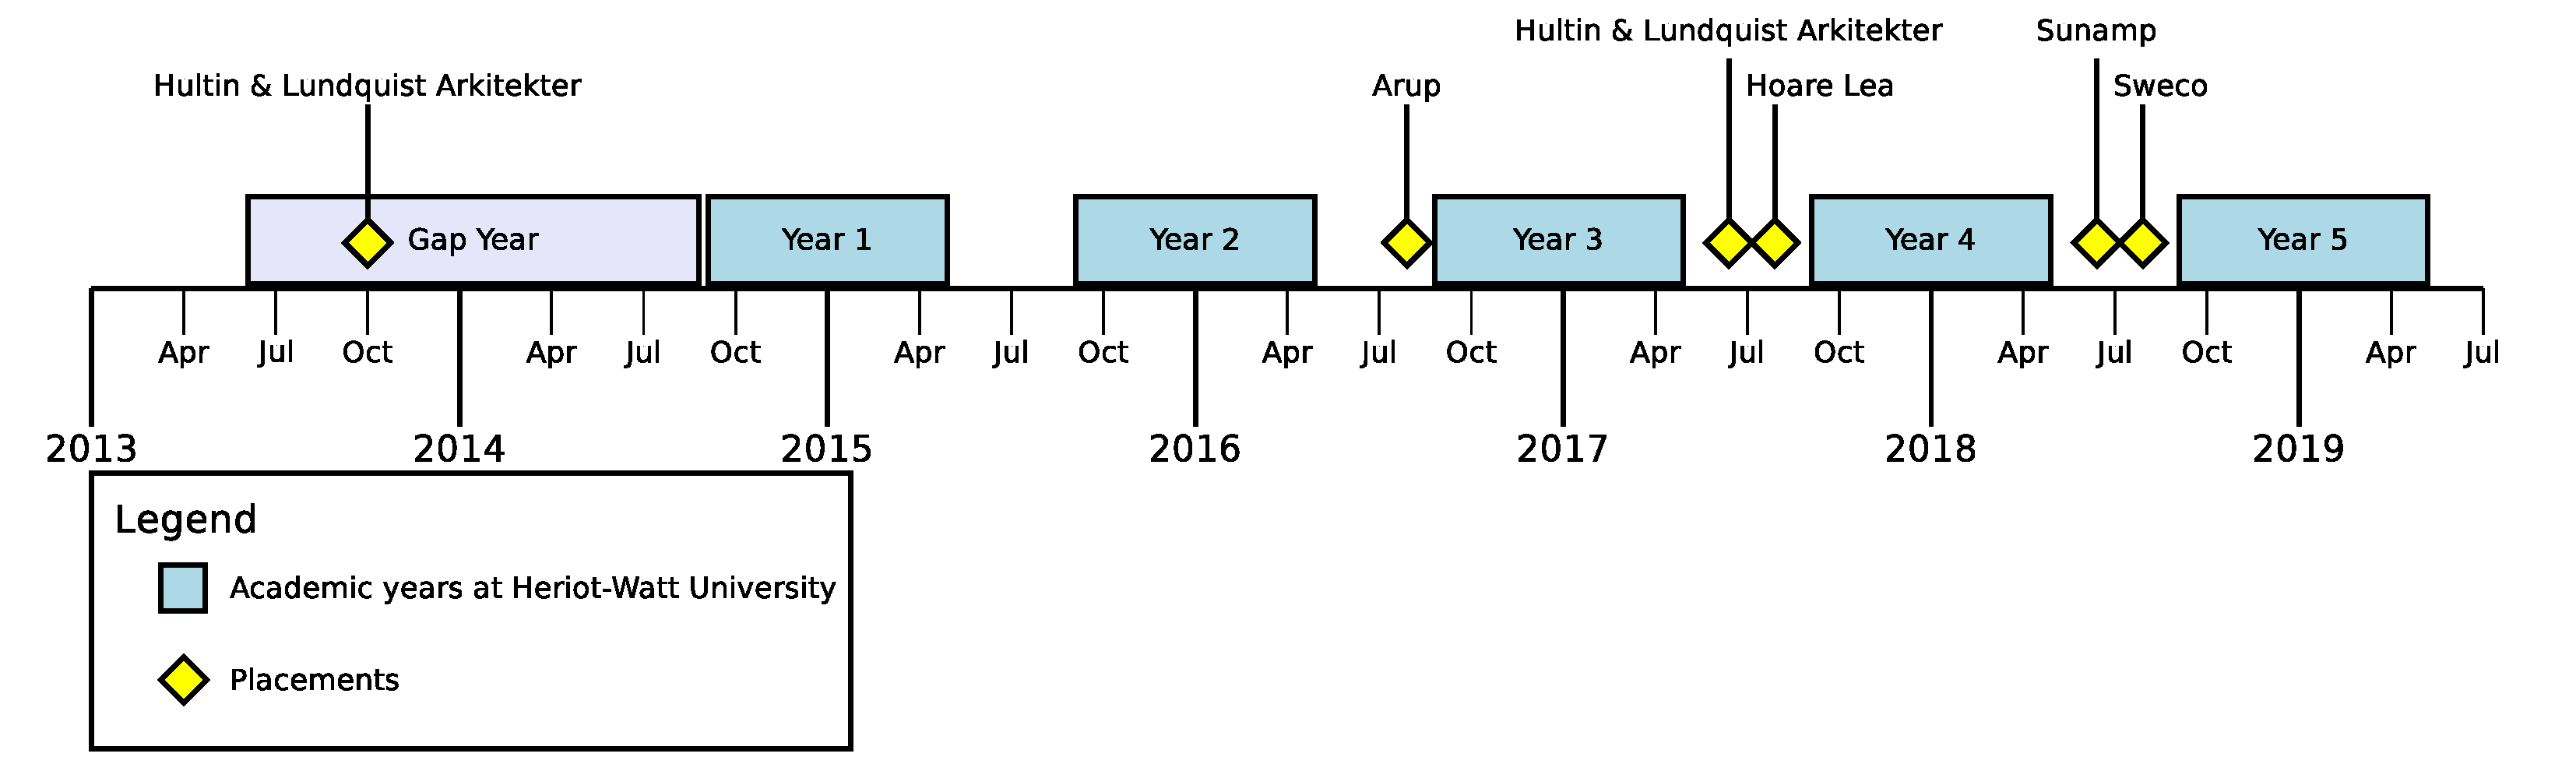
\includegraphics[width=\textwidth]{figures/IP-Timeline.eps}
	\rule{\textwidth}{0.5pt} % use line???
	\caption{Timeline of my work placements since my pre-university gap year.}
	\label{timeline}
\end{figure}


%----------------------------------------------------------------------------------------
%	SECTIONS
%----------------------------------------------------------------------------------------


%----------------------------------------------------------------------------------------
%	SECTION 1
%----------------------------------------------------------------------------------------


\section{Hultin \& Lundquist Arkitekter, October - December 2013}

%\subsection{Architecture Placement at Hultin \& Lundquist Arkitekter in Malm\"o, Sweden}

During the first half of my gap year, which I spent in Sweden, I was keen to gain work experience in architecture. I applied to all the architectural companies I could find in the Yellow Pages, with help from \textit{Ung Vision} (Young Vision).
\textit{Ung Vision} is a local initiative funded by Svedala council
%\footnote{\href{https://www.svedala.se/}{svedala.se}} 
with support from \textit{Arbetsf\"ormedlingen} (the Swedish Public Employment Service)
%\footnote{\href{https://www.arbetsformedlingen.se/Globalmeny/Other-languages/Languages/English-engelska.html}{arbetsformedlingen.se in English}} 
and \textit{F\"orsäkringskassan} (the Swedish Social Insurance Agency)
%\footnote{\href{https://www.forsakringskassan.se/privatpers/!ut/p/z1/04_Sj9CPykssy0xPLMnMz0vMAfIjo8ziTTxcnA3dnQ28LdyNTQ0cAwMMjU38jby8gg30w_Wj9KOASgxwAEcD_YLsbEUAFUIRCA!!/dz/d5/L0lDUmlTUSEhL3dHa0FKRnNBLzROV3FpQSEhL2Vu/?keepNavState=true}{forsakringskassan.se in English}} 
that aims to help unemployed people between the ages of 16 and 24 find work \citep{ungvision:online}.
I eventually managed to get myself a ten-week paid placement at Hultin \& Lundquist Arkitekter, a small architectural practice in Malm\"o which at the time consisted of two architects.

Working with buildings was very exciting for me; I would walk proudly with my clipboard, floor plan drawings and ruler to the 1960s apartment building the architects were going to refurbish.
I was responsible for correcting the measurements of the building's outdated architectural drawings.
I learned some of the rules used in architectural drawings and also gained some 2D modelling skills in  AutoCAD.
One of the things that still stands out to me today was how the building layout responded to the needs of the occupants in the 1960s.
Many flats had two entrances, which puzzled me until I was told that the larger door was the main entrance and the smaller a discreet `back' entrance for the servants.
Such nuggets of history that explained the purpose behind design was the beginning of my learning how design should be purposeful.
It also influenced me to apply for an architecture-related programme at university.

%----------------------------------------------------------------------------------------
%	SECTION 2
%----------------------------------------------------------------------------------------

\section{Arup, August 2016}

%\subsection{Mechanical Engineering Summer Placement at Arup in Leeds}

In the summer after second year, I was excited to have earned a mechanical engineering placement with the world-renowned company, Arup, in Leeds' Buildings team.
I was responsible for sizing ducts and pipes and for producing the RIBA Stage 3\footnote{Of the Royal Institute of British Architects (RIBA) Plan of Work 2013.}
layouts and schematics of a new-build’s ventilation, heating and domestic water systems (see Figure \ref{fig:arup_schematics}).
This placement gave me my first hands-on experience in designing and sizing such systems.
I appreciated the level of responsibility (and its associated challenge) that I was given since Day 1.
I was also introduced to some of the work the electrical engineers did.

The work experience prepared me for future courses such as \textit{Electrical and Lighting Services for Buildings} and the 4\textsuperscript{th} year \textit{Design Project}.
I was encouraged to hear about Arup's sustainable mindset to designing and felt like I could become competent and may enjoy a job as a consulting engineer in the future.


\begin{figure}[htbp]
	\centering
	\begin{subfigure}[b]{0.48\textwidth}
		\includegraphics[width=\textwidth]{figures/VentilationSchem3.PNG}
		\caption[Arup ventilation schematic.]{Ventilation schematic.}\label{fig:ventilation}
	\end{subfigure}
	
	\begin{subfigure}[b]{.48\textwidth}
		\centering
		\includegraphics[width=\textwidth]{figures/HeatingSchem.PNG}
		\caption[Arup heating schematic.]{Heating schematic.}\label{fig:heating}
	\end{subfigure}
	\begin{subfigure}[b]{.48\textwidth}
		\centering
		\includegraphics[width=\textwidth]{figures/DomesticsSchem.pdf}
		\caption[Arup domestic schematic.]{Domestic water services schematic.}\label{fig:domestic}
	\end{subfigure}
	\rule{\textwidth}{0.5pt} % use line???
	\caption{Schematics produced at Arup.}
	\label{fig:arup_schematics}
\end{figure}

%----------------------------------------------------------------------------------------
%	SECTION 3
%----------------------------------------------------------------------------------------

\section{Hultin \& Lundquist Arkitekter, June 2017}

%\subsection{Architecture Placement at Hultin \& Lundquist Arkitekter in Malm\"o, Sweden}
During my second placement at Hultin \& Lundquist Arkitekter, I:
\begin{itemize}
	\item Produced window, door and kitchen schedules on AutoCAD.
	\item Was responsible for daylight calculations of a new-build during planning stage.
	\item Began a feasibility study on the construction of recycling sheds to five existing apartment buildings shortly before the end of my placement.
\end{itemize}

%How did I progress or what did I learn during this placement?
I had to be creative in clearly displaying the numbers and types of doors, kitchens and apartments in schedules.
I achieved this through the use of tables, as seen in Figure \ref{fig:schedules}.
I also improved my conditional formatting skills in spreadsheets during my work on daylight calculations.
%Practised my 2D AutoCAD skills again.
%Took measurements to double-check the accuracy of outdated drawings.
%Apart from these things which were somewhat stimulating, I found the tasks I was given a bit monotonous.

\begin{figure}[htbp]
	\centering
	\begin{subfigure}{.48\textwidth}
		\centering
		\includegraphics[height=4cm]{figures/door-schedule.png}
		%          \rule{\textwidth}{0.5pt} % use line???
		\caption{Door schedule}
		\label{fig:sched_doors}
	\end{subfigure}
	\begin{subfigure}{.48\textwidth}
		\centering
		\includegraphics[height=4cm]{figures/kitchen-schedule.png}
		%          \rule{\textwidth}{0.5pt} % use line???
		\caption{One of the kitchen schedules}
		\label{fig:sched_kitchen}
	\end{subfigure}
	\rule{\textwidth}{0.5pt} % use line???
	\caption[Hultin \& Lundquist Arkitekter schedules.]{Screenshots of schedules done in AutoCAD at Hultin \& Lundquist Arkitekter.}
	\label{fig:schedules}
\end{figure}

%----------------------------------------------------------------------------------------
%	SECTION 4
%----------------------------------------------------------------------------------------

\section{Hoare Lea, August 2017}

%\subsection{Electrical Engineering Summer Placement at Hoare Lea in London}

Having recently studied \textit{Electrical and Lighting Services for Buildings} and already tried out mechanical engineering at Arup, I wanted to explore the other half of M\&E.
I got the opportunity to explore electrical engineering at Hoare Lea, a building services consultancy, in their London office.
%Just preparing for my interview for the Hoare Lea placement made me take some time to reflect on skills and attributes.
%It also improved on my presentation-making skills.
Some of the tasks I got to do are:
\begin{itemize}%
	\item Produce RIBA Stage 3 layouts and schematics of electrical and fire detection and alarm installations for a new-build. These were made to comply with standards e.g. BS 5839-8:2013.
	\item Assist the Building Information Modelling (BIM) department with coordination work on Revit.
\end{itemize}

I enjoyed drawing the fire detection and alarm drawings, which was an unfamiliar exercise to me.
I learned a lot from two fire specialists from Honeywell, who guided me through the design exercise and to the relevant technical documentation.

Unfortunately due to having not-so-engaged supervisors, I do not think I learned as much about electrical engineering as I could have and would have liked.

%I practised drawing an electrical schematic by hand, on AutoCAD and on Amtech.
%Despite not doing much, I did learn a bit about busbars, lighting and resilient cables.



The London office housed many different disciplines.
I therefore took the opportunity to `roam' around and explore the different types of work that I could get into after university.
I was introduced to eight different specialities:
electrical engineering,
fire engineering,
building optimisation,
BIM,
acoustics,
sustainability,
façade access and
vertical transportation.
I was excited to learn about the breadth of career opportunities within building services.
I gained particular interest in the building optimisation speciality where one analyses the modelled and actual performance of buildings, advises clients on how to optimise the performance of their building and reduce running costs.
I would say my experience at Hoare Lea broadened rather than deepened my knowledge in AE.
Thanks to my exposure to these specialities, I have been able to discover new and exciting career paths, of which I am considering working in building optimisation (for more about this, go to Section~\ref{sec:future}).

%----------------------------------------------------------------------------------------
%	SECTION 5
%----------------------------------------------------------------------------------------

\section{Sunamp, July - August 2018} \label{sec:sunamp}


\subsection*{The Company}

% copied and pasted from Susan's emails %

Sunamp designs and produces super-compact heat batteries which store available energy as heat and release it when it is required, thus overcoming the intermittent nature of many other renewable energy sources.
The technology is based on phase change materials (PCMs) to provide a clean, efficient and cost-effective heat energy storage solution.


Working with multiple energy sources including solar and heat pumps, the company’s UniQ range of heat batteries has the potential to make conventional hot water cylinders obsolete and delivers cascades of hot water and highly responsive space heating with proven savings of up to 75\% on utility bills.
The technology offers limitless scalability for residential, commercial or industrial projects.


% % % % % % % % % %


%Sunamp is a newly established business that specialises in the research, production and sales of heat batteries that are based on phase change materials (PCMs).
The PCMs, developed and manufactured by Sunamp, are non-toxic, non-flammable, eco-friendly and patented in the UK and China, with patents pending in other countries \citep{SunampAutomotive}.
The PCMs operate at different temperatures, allowing the storage of heat (up to 1000$^{\circ}$C) or coolth (less than 0$^{\circ}$C) (see Figure~\ref{pcm_temp_range}).
Currently, the company's main markets are buildings, where their heat batteries can generate hot water and space heating, and automobiles, where their heat batteries can refrigerate transported goods (for example).

\begin{figure}[htbp]
	\centering
	\includegraphics[width=\textwidth]{figures/temperature-range-of-PCMs.jpg}
	\rule{\textwidth}{0.5pt} % use line???
	\caption{The temperature range of Sunamp's PCMs in degrees Celsius \citep{SunampAutomotive}.}
	\label{pcm_temp_range}
\end{figure}


Sunamp was founded by Andrew Bissell, who is the chief executive officer (CEO).
In Macmerry, East Lothian, they have an office building which features a research and development (R\&D) workshop and materials laboratory on the ground floor and an open-plan office on the first floor.
They also have a factory across the road where they have additional test facilities but primarily do large-scale manufacturing %and packaging 
of heat batteries.
Sunamp employs 32 people: 22 office-based, six in the factory, three based on the road and one based in Zurich, where Sunamp has a small satellite office.





%%%%%%%%%%%%%%%%%%%%%%%%%%%
\subsection*{Their Products}

\begin{wrapfigure}{r}{0.3\textwidth}
	\includegraphics[width=0.3\textwidth]{figures/sunamp-hand-warmer.png}
	\rule{0.3\textwidth}{0.5pt} % use line???
	\caption{A crystallising hand warmer \citep{FullyCharged}.}
	\label{fig:handwarmer}
\end{wrapfigure}

If you have ever gone camping, you might have come across crystallisation-type reusable hand warmers (pictured in Figure~\ref{fig:handwarmer}).
Such hand warmers are filled with a PCM called sodium acetate and contain a little metal disk.
The sodium acetate is liquid at room temperature.
When you bend the metal disk, the sodium acetate gradually crystallises and releases heat 
(see a video of the crystallisation process here: 
\url{https://upload.wikimedia.org/wikipedia/commons/0/09/Hand_warmer_activation.webm} \citep{HandWarmerActivation}).
The pack becomes completely solid and continues to release heat for a while.
The hand warmer is reusable because you can turn the sodium acetate back into a liquid by immersing the pack in boiling water for about ten to 15 minutes.

The principle that makes hand warmers work is \emph{latent heat}.
Latent heat is the thermal energy required to change the phase of a substance (e.g. from a solid to a liquid, or a liquid to a gas) without it changing temperature (see Figure~\ref{fig:latentheat}).
Latent heat can be thought of as the energy required to make or break the molecular bonds within a substance, thereby changing its state.


\begin{figure}[htbp]
	\centering
	\begin{subfigure}{.49\textwidth}
		\centering
		\includegraphics[width=\textwidth]{figures/LatentHeatStorage.eps}
		%          \rule{\textwidth}{0.5pt} % use line???
		\caption{Latent heat storage}
		\label{fig:latentheatstorage}
	\end{subfigure}
	\begin{subfigure}{.47\textwidth}
		\centering
		\includegraphics[width=\textwidth]{figures/LatentHeatEmission.eps}
		%          \rule{\textwidth}{0.5pt} % use line???
		\caption{Latent heat emission}
		\label{fig:latentheatemission}
	\end{subfigure}
	\rule{\textwidth}{0.5pt} % use line???
	\caption[Graphical representations of latent heat.]{Graphical representations of latent heat (slightly adapted from \EnBldgsTitle \space lecture slides \citep{jenkins}).}
	\label{fig:latentheat}
\end{figure}


%For example, take a PCM that melts at 58$^{\circ}$C.
Water is an example of a PCM.
%Water freezes at 0$^{\circ}$C, and in reverse, ice melts at 0$^{\circ}$C.
When you put water in a cold environment, like a freezer, it exchanges heat with the environment: the water loses latent heat and becomes solid ice at 0$^{\circ}$C, and the environment gains heat, becoming somewhat warmer.
When you put the solid ice in a warm environment, the reverse happens: the ice gains latent heat and becomes liquid water at 0$^{\circ}$C, and the environment loses heat, becoming somewhat cooler.
%When you put ice in a warm environment, it exchanges heat with the environment: the ice gains latent heat and becomes liquid water at 0$^{\circ}$C, and the environment loses heat, becoming somewhat cooler.
%When you put the liquid water back in a cold environment such as a freezer, the reverse happens: the water loses latent heat and becomes solid ice at 0$^{\circ}$C, and the environment gains heat, becoming somewhat warmer.

%Sunamp's heat batteries are ``scaled up" versions of crystallisation-type hand warmers.
%They charge (i.e. absorb heat) when heat is added to the battery, e.g. via piped hot water running through the battery or via an electrical heating element inside the battery.
%They then discharge (i.e. release heat) when piped cold water runs through the battery, thereby exchanging heat with the water.
%The hot water that is discharged from the battery can be used for space heating and hot water purposes in buildings.


\begin{figure}[htbp]
	\centering
	\begin{subfigure}{.24\textwidth}
		\centering
		\includegraphics[width=\textwidth]{figures/sunamp-uniq-3.png}
		%          \rule{\textwidth}{0.5pt} % use line???
		\caption{UniQ 3\\
			(3.5 kWh)}
		\label{fig:uniq3}
	\end{subfigure}
	\begin{subfigure}{.24\textwidth}
		\centering
		\includegraphics[width=\textwidth]{figures/sunamp-uniq-6.png}
		%          \rule{\textwidth}{0.5pt} % use line???
		\caption{UniQ 6\\
			(7.0 kWh)}
		\label{fig:uniq6}
	\end{subfigure}
	\begin{subfigure}{.24\textwidth}
		\centering
		\includegraphics[width=\textwidth]{figures/sunamp-uniq-9.png}
		%          \rule{\textwidth}{0.5pt} % use line???
		\caption{UniQ 9\\
			(10.5 kWh)}
		\label{fig:uniq9}
	\end{subfigure}
	\begin{subfigure}{.24\textwidth}
		\centering
		\includegraphics[width=\textwidth]{figures/sunamp-uniq-12.png}
		%          \rule{\textwidth}{0.5pt} % use line???
		\caption{UniQ 12\\
			(14 kWh)}
		\label{fig:uniq12}
	\end{subfigure}
	\rule{\textwidth}{0.5pt} % use line???
	\caption{Sunamp's UniQ heat battery range and nominal heat storage capacities in kWh \citep{SunampHomepage}.}
	\label{fig:uniq_range}
\end{figure}


Sunamp's latest range of heat batteries is called \emph{UniQ} (see Figure~\ref{fig:uniq_range}).
Why?
\emph{Uni} because it is the ``one and only energy storage solution you need for" \emph{Q}, the ``engineering symbol for Heat Energy" \citep{UniQ_Leaflet}.
The UniQ batteries are ``scaled up" versions of crystallisation-type hand warmers.
There are two series of UniQ batteries: standard batteries and e-batteries.
Broadly speaking, a standard UniQ battery consists of a highly insulated box which contains a finned-tube heat exchanger and a PCM which fills the space around the heat exchanger (see cross-section in Figure~\ref{fig:uniq_cross-section}).
The tubes of the heat exchanger protrude from the box, allowing pipe connections to serve as hot and cold water inlets to the battery, as well as hot water and space heating outlets from the battery.
A UniQ e-battery has a similar construction, except it also contains an electrical heating element (see Figure~\ref{fig:euniq_cross-section}).
A battery charges (i.e. its PCM absorbs heat) when heat is added to it, e.g. via piped hot water running through a standard battery or by switching on the electrical heating element inside an e-battery.
A battery then discharges (i.e. its PCM releases heat) when piped cold water runs through it, the warm PCM thereby exchanging heat with the cold water.
The hot water that is discharged from the battery can be used for space heating and hot water purposes in buildings.


\begin{figure}[htbp]
	\centering
	\begin{subfigure}{.48\textwidth}
		\centering
		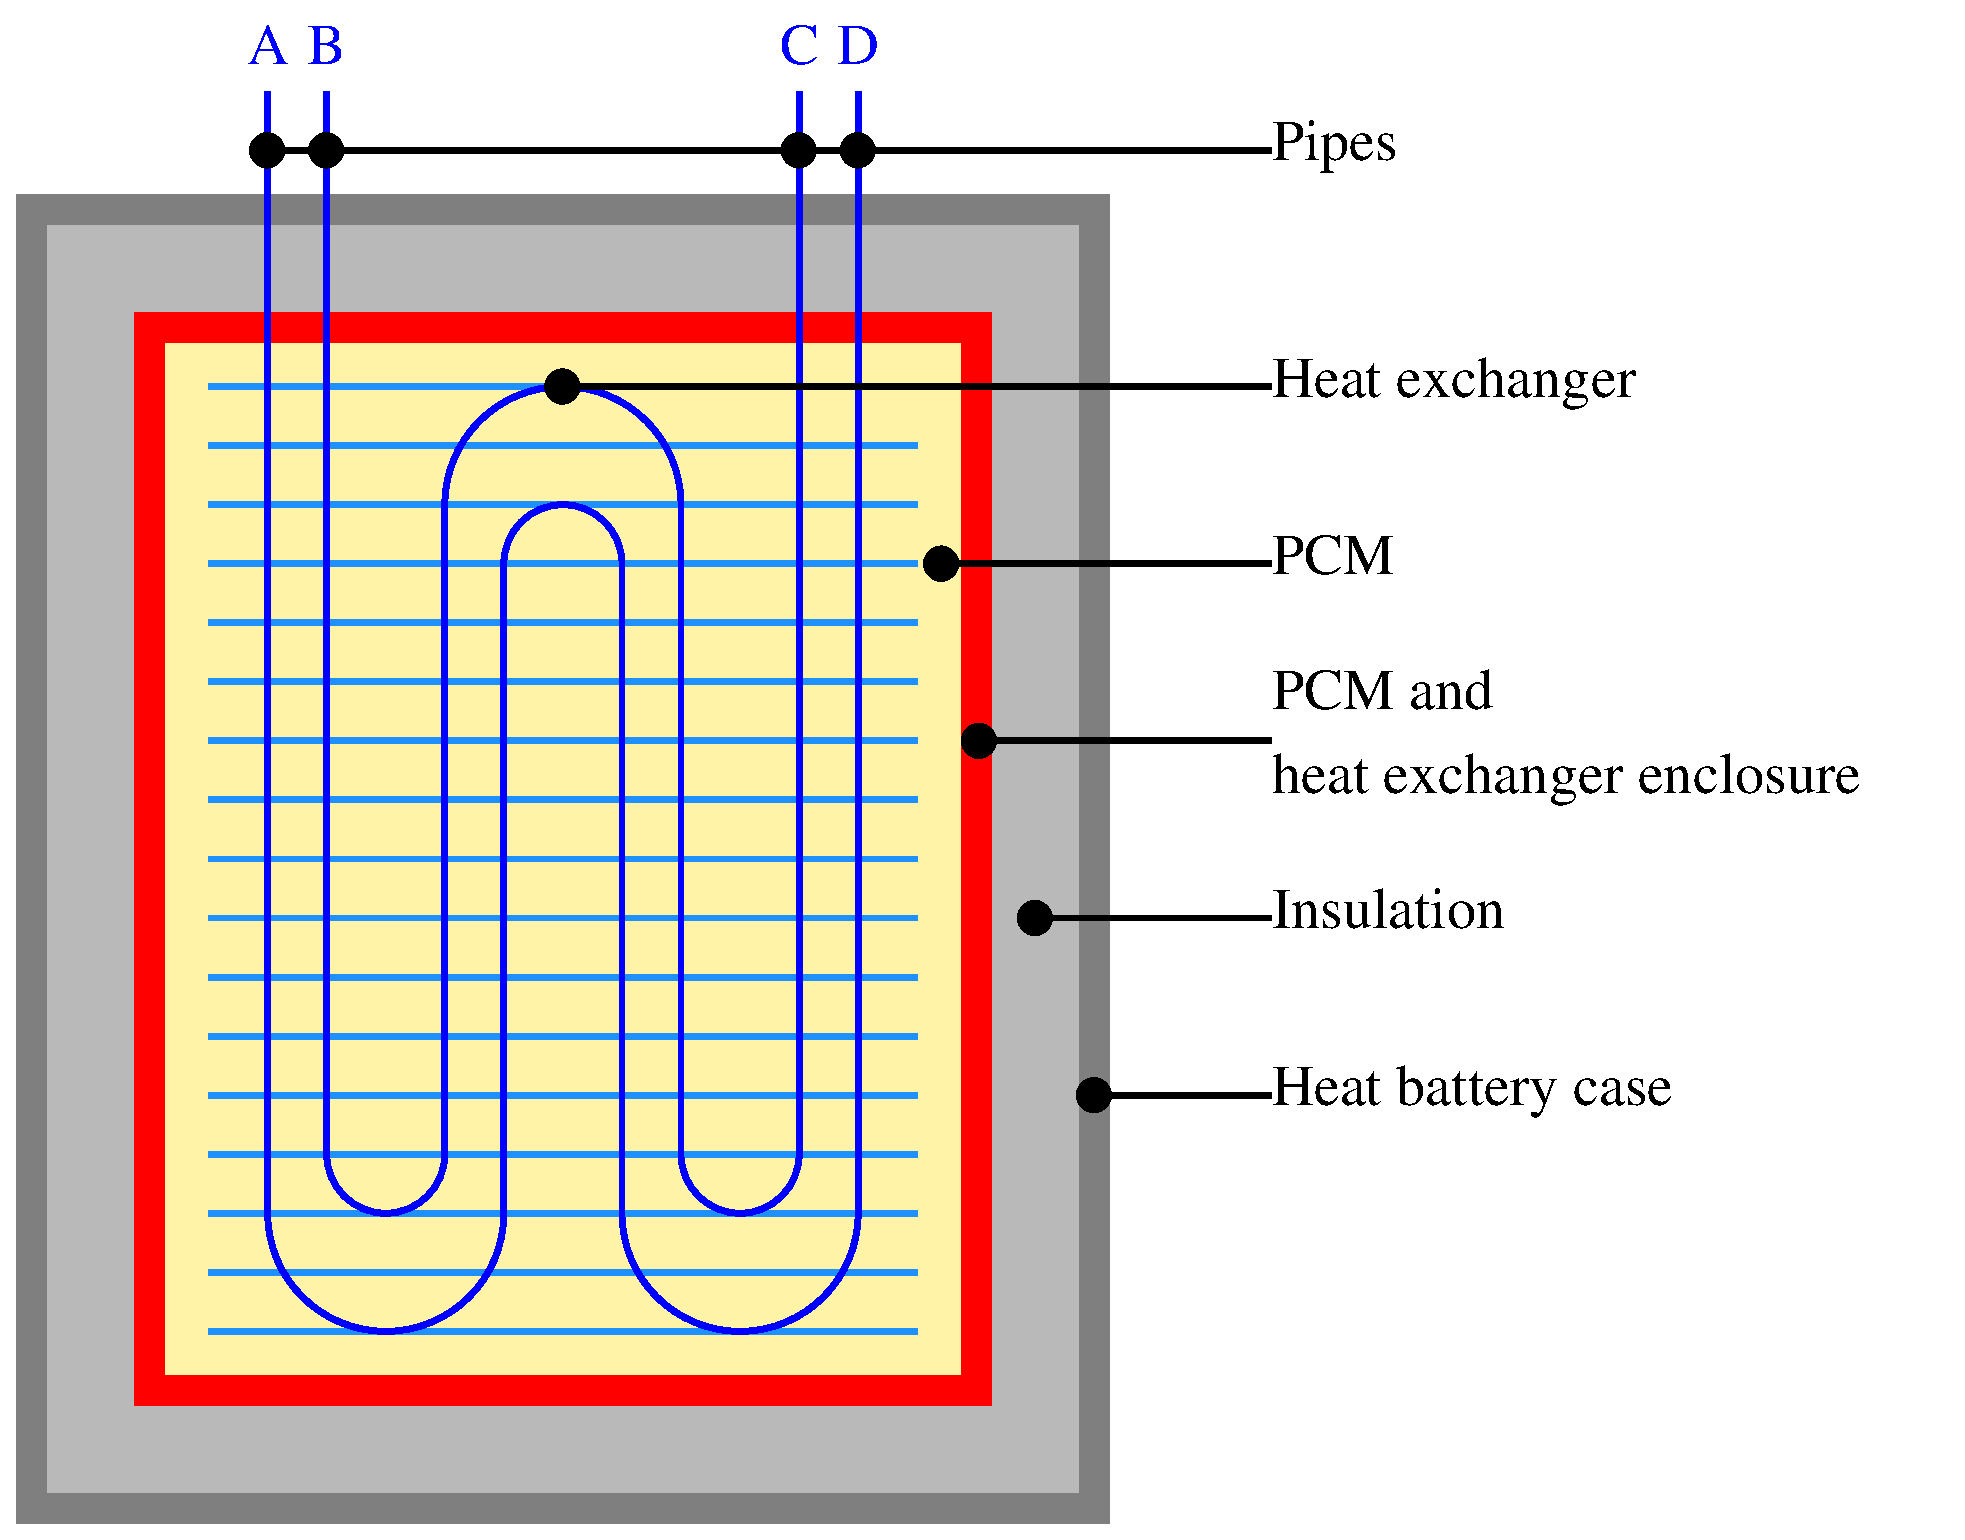
\includegraphics[width=\textwidth]{figures/UniQ_std_cross-section.eps}
		%          \rule{\textwidth}{0.5pt} % use line???
		\caption{Standard UniQ battery}
		\label{fig:uniq_cross-section}
	\end{subfigure}
	\begin{subfigure}{.48\textwidth}
		\centering
		\includegraphics[width=\textwidth]{figures/eUniQ_cross-section.eps}
		%          \rule{\textwidth}{0.5pt} % use line???
		\caption{UniQ e-battery}
		\label{fig:euniq_cross-section}
	\end{subfigure}
	\rule{\textwidth}{0.5pt} % use line???
	\caption{Cross-sections of Sunamp's UniQ batteries.}
	\label{fig:cross-sections}
\end{figure}


%%%%%%%%%%%%%%%%%%%%%%%%%%%
\newpage
\subsection*{Why Heat Batteries?}

\begin{wrapfigure}{r}{0.4\textwidth}
	\includegraphics[width=0.4\textwidth]{figures/household-energy-consumption.jpg}
	\rule{0.4\textwidth}{0.5pt} % use line???
	\caption{Typical energy consumption of a UK home \citep{SunampResidential}.}
	\label{fig:domestic-energy}
\end{wrapfigure}

Electric batteries like the Tesla Powerwall have gained a lot of media attention recently for being able to store renewable electricity and shift demand etc.
However, in the UK (and probably other countries with a similar climate), over 80\% of domestic energy is used to generate heat for space heating and hot water (see Figure~\ref{fig:domestic-energy}).
Considering that the majority of UK households generate heat from natural gas, and some from fossil fuelled electricity, that causes a large carbon footprint.
Moreover, the current heat storage solutions are not as effective as they could be.
For example, in my flat, I have a direct hot water cylinder which turns on early every morning so that I have hot water as soon as I wake up.
But by the evening, the water is lukewarm or cold and, if I require any more hot water, I need to use more electricity to boost the hot water cylinder.
The poor heat storage capacity of my cylinder is probably due to its poor insulation, but perhaps also due to the relatively low heat capacity of water.
For a sustainable future, we need to be smarter about the way we generate and use heat, which is something we are evidently highly dependent on.




Sunamp’s UniQ heat batteries offer a smart solution to sustainable heat generation and consumption.
%Due to the high specific heat capacity of their PCMs, problems such as me re-boosting my hot water cylinder can be avoided.
%OR 
Due to the high heat capacity of their PCMs\footnote{
	I do not know the heat capacity of Sunamp's PCMs, but to get an idea, the heat capacity of sodium acetate can be as high as 229 $J/mol \cdot K$ \citep{Csodiumacetate} whereas that of water is 69.95 $J/mol \cdot K$ \citep{Cwater} according to the National Institute of Standards and Technology (NIST).
} and the low heat losses of their batteries, an excessive amount of energy does not need to be used to generate or store heat (cf. my aforementioned hot water cylinder example).
Moreover, their heat batteries can be charged by any energy source, including renewable and/ or environmentally friendly technologies such as PVs and heat pumps. %, which are energy generation solutions for a sustainable future.
%Furthermore, with thoughts to electrify heat in the UK (as grid electricity gradually becomes decarbonised), 
UniQ e-batteries also allow for demand-side management (DSM) which helps with grid balancing, e.g. by shifting electricity demands from peak periods, thus reducing the strain on the national electricity supply system (see Figure~\ref{fig:DSM}).
DSM might become an increasingly important strategy since there have been thoughts to electrify heat in the UK as grid electricity gradually becomes decarbonised.




\begin{wrapfigure}[3]{r}{0.2\textwidth}
	\centering
	\begin{subfigure}{.2\textwidth}
		\centering
		\includegraphics[width=\textwidth]{figures/DSM-base.png}
		%          \rule{\textwidth}{0.5pt} % use line???
		%\caption{Latent heat storage}
		%\label{fig:latentheatstorage}
	\end{subfigure}
	\begin{subfigure}{.2\textwidth}
		\centering
		\includegraphics[width=\textwidth]{figures/DSM-load-shift.png}
		%          \rule{\textwidth}{0.5pt} % use line???
		%\caption{Latent heat emission}
		%\label{fig:latentheatemission}
	\end{subfigure}
	\rule{0.2\textwidth}{0.5pt} % use line???
	\caption[Load shifting, an example of DSM.]{Load shifting, an example of DSM \citep{USAID}).}
	\label{fig:DSM}
\end{wrapfigure}

Other key features of UniQ batteries include:
\begin{itemize}
	\item Instant hot water at mains pressure
	\item Rapid warm-up of your heating system, e.g. radiators
	\item Significantly reduced legionella risk, since there is hardly any risk of water stagnating or being between 20$^{\circ}$C and 45$^{\circ}$C inside the battery \citep{HSE_legionella}
	\item Compact, between two and four times smaller than the equivalent hot water cylinders
	\item Reliable, with a lifespan of at least 50 years
	\item Modular: the batteries can easily be combined to increase heat storage
	\item You can save money by charging your e-battery during off-peak periods with variable rate electricity tariffs, e.g. Economy 10
\end{itemize}



%%%%%%%%%%%%%%%%%%%%%%%%%%%

\subsection*{Description of Work Experience}

\begin{wrapfigure}{r}{0.4\textwidth}
	\includegraphics[width=0.4\textwidth]{figures/bridge.png}
	\rule{0.4\textwidth}{0.5pt} % use line???
	\caption{My place at Sunamp.}
	\label{fig:bridge}
\end{wrapfigure}

My placement at Sunamp started on Tuesday 3\textsuperscript{rd} July 2018 and ended on Friday 10\textsuperscript{th} August 2018.
I worked a total of 198 hours across six weeks, averaging at about 6.8 hours of work per day (see log in Appendix~\ref{App:Log}).

I joined Sunamp in the wake of the development of UniQ.
UniQ had been developed by Sunamp's engineers and explained in a manual.
However, the manual was too large and technical for the sales team to understand, navigate and use to efficiently match customers with the most suitable UniQ products.
Therefore, my purpose at Sunamp was to bridge the gap between Engineering and Sales (see Figure~\ref{fig:bridge}).
This was to be done by creating concise and user-friendly documentation that would introduce and explain the UniQ range to customers and even be used by the sales team as an aide-memoire.
This project mainly consisted of me presenting existing content in new ways and boiling down a lot of technical documentation/ material into meaningful and useful information for customers.

My time at Sunamp can roughly be divided up into two aspects: learning about Sunamp's work and development, and
% \hl{producing work for Sunamp/ }
carrying out my UniQ project.




%-----------------------------------
%	SUBSECTION 1
%-----------------------------------

\subsection{Learning About Sunamp}

The majority of my first week at Sunamp consisted of my familiarisation with the company and their products.
The week started with an induction from Susan Lang-Bissell, the Chief Operation Officer (COO), where we went over my contract, office information, health and safety regulations (amongst other things) and I got a brief tour of the factory.
The induction was followed by an introduction from Joan Pisanek (the Business Development Manager) to UniQ and some of Sunamp's projects.
I used the rest of the week to familiarise myself with and try to understand their products by consulting Joan's PowerPoint presentations and the UniQ manuals,
% working through Joan's Buchlyvie project (\hl{see Appendix ...}),
and attempting a UniQ Product Training Exercise developed by Sandy.

Santokh Gataora, colloquially known as Sandy, is Sunamp's Technical Director.
He has a vast experience in building services engineering and has helped develop the UniQ product range.
He writes and continues to refine the UniQ manuals as he guides the company in the engineering and application aspects of UniQ heat batteries in buildings.
% When I joined the company, UniQ was a very recent development that the sales team was still learning about.
% The week I arrived at Sunamp, Sandy had sent out an exercise for the sales team to complete for the following week's UniQ Product Training Workshop.
% The exercise instructions and my answer \hl{can be found in Appendix ... blur out people's names in email}.
During my second week, I attended the UniQ Product Training Workshop, where the sales team and I learned about the UniQ product range in greater depth and briefly went over the solution to the aforementioned exercise.
%\hl{Comment on my answer vs. solution?}

During my second and third weeks at Sunamp, I received more thorough tours of the factory, workshop and chemistry laboratory.
At the factory I got an understanding of the construction of the heat batteries.
I touched a heat battery that had been assembled some days before and left to cool off; it was \emph{still warm} -- I was amazed by its impressively low heat losses!

During the workshop and laboratory tour, I gained a deeper understanding of the making and performance of the PCMs and the selection of materials that go inside a heat battery.
Some of the things I learned are:
\begin{itemize}
    \item The high energy density of the PCMs is what allows Sunamp's heat batteries to be between two and four times smaller than their equivalent hot water cylinders.
    \item Sunamp's chemists cycle and analyse PCM mixtures through solid-liquid and liquid-solid phase transitions to assess the stability of the mixtures' phase transitions over time. The more stable the transitions are, the more suitable they are to be used in heat batteries.
    %\item The chemists also need to test their supplier's materials for impurities which can significantly degrade the performance of PCM mixtures.
    \item Different PCM mixtures can react differently to aluminium and copper, the main metals that heat exchangers are built from.
    Sunamp typically uses all-aluminium finned-tube heat exchangers, but they will sometimes create a PCM which corrodes aluminium.
    In these cases they might need to consider using copper-based heat exchangers, which are more expensive but might work out cheaper in the long-run when compared to the capital and operational costs of the heat batteries' equivalent hot water cylinders.
    \hl{just refer back to your temperature chart and it will make sense and be less alarming}
    %\item Working with cold, medium and high temperature ranges, the chemists need to ensure that the plastic material of the container which holds the PCM can tolerate that PCM's temperature range. Therefore Sunamp typically uses different materials for containers that carry cold and warm/ hot PCMs.
\end{itemize}

During my fourth and fifth weeks at Sunamp, I attended two presentations.
The first was a summary of the research carried out by two chemistry students that had spent the past year working on their dissertation projects at Sunamp.
I gained some insight into the technical aspects of the development of PCMs and was impressed that one of the student's PCMs might soon become patented and used for refrigeration in vehicles.
Sandy gave the second presentation which was an overview of the new UniQ product range to the whole company.
I think this was especially insightful for the chemists and engineers who are specialised in their specific areas and might not always see how all of their work contributes to the end-product (heat batteries) and their application (heating space and water in buildings).

During my last week, I was part of the tour and planning of Sunamp's Experience Room.
This room is designed to look and feel like a home, with a kitchen-like decor and sink in one corner.
One of the purposes of this room, which was still under construction, is to showcase Sunamp's heat batteries to customers by comparing them to their large equivalents on the common marketplace (e.g. hot water cylinders) and by showing how they integrate into a building and its systems (e.g. heat pumps
and boilers).
The room is also planned to be used for training workshops on the installation of Sunamp's heat batteries.

Throughout my brief placement at Sunamp, there has been a sense of rapid development and expansion.
The company started out by manufacturing batteries inside a small workshop, which has now grown into a factory which is still evolving with the construction of new testing facilities and training/ marketing spaces.
The company continues to recruit more engineers and scientists.
It also seems like more customers are hearing about and taking interest in Sunamp's heat batteries, in the UK and abroad.

%\hl{See notebook notes on how to demonstrate technical understanding.}




%-----------------------------------
%	SUBSECTION 2
%-----------------------------------

\subsection{My UniQ Project} \label{sec:sunamp_work}

%\hl{Decide on section title!}

% Ohhhh come on! I gotta write! Just blow off some steam. It doesn't have to be all thought out and structured to begin with. Just keep the hand on the keyboard and type! As Moira says, "Be confident." :D

I started working on my project during my second week at Sunamp and completed it during my last week.
From my log, I have deducted that I worked at least 138 hours on this project, which accounts for 70\% of my time at Sunamp.
This includes the time I spent working autonomously, in meetings, and my final presentation.

I ended up creating a series of documents about UniQ, most of which are illustrated in Figure~\ref{funnel}.
The documents formed a hierarchy, from very generic information at the top to more specific information going down.
This funneling of information reflects the customer's journey, from the time they become aware of a product until they decide to purchase it.
\hlc[cyan]{
When I was preparing for my presentation, I discovered that my funnel resembles a marketing strategy/ concept called the marketing funnel.
This starts out by making customers aware of the product and then increasingly provides more specific information as a customer becomes more interested until they decide to purchase the product.}
\hlc[green]{On reflection...
This corroborated/ validated my use of the funnel.}
At the top of the funnel were documents that introduced and gave an overview of the UniQ product range.
These consisted of the Overview Sheet and UniQ Product Selection Quiz.
At the next level of the funnel were documents that provided specific information about the individual UniQ products; these were called the Product Information Sheets (PISs).
At the bottom of the funnel was a document that provided installation guidelines for the UniQ batteries.


\begin{figure}[htbp]
	\centering
	\includegraphics[width=\textwidth]{figures/Funnel.PNG}
	\rule{\textwidth}{0.5pt} % use line???
	\caption{The main outcomes of my UniQ project, ranked by a funnel-shaped hierarchy.}
	\label{funnel}
\end{figure}


Outside the heart of my project, embodied by the information funnel in Figure~\ref{funnel}, I carried out a couple other tasks.
Among these was \hl{a document} I produced that contained additional information that was to be included in Sunamp's upcoming UniQ brochure.
Also, at the end of my placement, I gave a presentation to Sunamp's core staff, including the CEO, about my placement work.

The following sections will discuss my work in more detail.



\subsubsection{UniQ Overview Sheet}

I had not been asked to create a sheet that gave an overview of the UniQ product range.
I, however, thought it might be helpful to ease the customers' introduction to and understanding of UniQ.
The final Overview Sheet (see Appendix~\ref{App:Overview}) introduces the UniQ battery by showing the possible inputs (renewables, heat and/ or electricity) and outputs (space heating and/ or hot water).
The battery is flexible when it comes to its inputs: these can range from boilers to heat pumps, and from grid electricity to PV panels.
Furthermore, the sheet features some catchy ways to describe UniQ, including the tag line ``Make your heating solution UniQ", that I came up with.
\hlc[green]{On reflection, the sheet misses the point of getting a heat battery. Why would I get a battery if I already have the means to generate space heating and hot water. I think this was raised during the meeting by Andrew and was to be rectified after I left.}

It turned out that Sunamp already had a diagram showing the inputs and outputs of a UniQ battery.
However, the staff considered using mine over their original diagram in the UniQ brochure.



\subsubsection{UniQ Product Selection Quiz} \label{sec:quiz}

As I was working on the PISs, the question of how a customer would know which UniQ product was most suitable to them \hl{loomed} in my mind.
``How will they even know which PIS to read?"
That is when I thought of creating a quiz in the form of a decision tree that would ask customers questions and guide them to the most suitable UniQ product for them based on their answers.
An added benefit of the quiz was that it would allow customers to explore the UniQ range easier and more informed, which would cut some of the sales team's initial \hl{customer-product match-making/ interface work}.

Figure~\ref{fig:quiz_draft} shows my first draft of the quiz.
I showed this to Joan when I pitched the quiz idea to her.
The idea was well received by her and Susan, so it escalated to another one of my sub-projects.
After creating a more polished second draft, I asked Sandy to give his expert feedback.
He responded with a re-arranged and more sophisticated decision tree.
This was the start of a process of iterations where I asked staff members for further feedback in order to refine the quiz design.
The full-sized version of the final quiz (Figure~\ref{fig:quiz_final}) can been found in Appendix~\ref{App:quiz}.


%\begin{figure}[htbp]
%	\centering
%	\includegraphics[width=0.5\textwidth]{figures/QuizSketch.png}
%	\rule{\textwidth}{0.5pt} % use line???
%	\caption{My first draft of the UniQ Product Selection Quiz.}
%	\label{quiz_draft}
%\end{figure}


\begin{figure}[htbp]
    \centering
        \begin{subfigure}{.38\textwidth}
          \centering
          \includegraphics[width=\textwidth]{figures/QuizSketch.png}
%          \rule{\textwidth}{0.5pt} % use line???
          \caption{First draft}
          \label{fig:quiz_draft}
        \end{subfigure}
        \begin{subfigure}{.58\textwidth}
          \centering
          \includegraphics[width=\textwidth]{Appendices/final_quiz.pdf}
%          \rule{\textwidth}{0.5pt} % use line???
          \caption{Final result}
          \label{fig:quiz_final}
        \end{subfigure}
    \rule{\textwidth}{0.5pt} % use line???
    \caption{The first draft and final result of the UniQ Product Selection Quiz.}
    \label{fig:quiz}
\end{figure}



\subsubsection{UniQ Product Information Sheets (PISs)} \label{sec:piss}

Sandy asked me to produce a PIS for each of the UniQ products.
He gave me an outline of the type of information that would be included on each sheet, e.g. a brief description of the product and its operation, a diagram, and battery sizing information.
%, hydraulic connections, a wiring diagram, and a ``Do's and Don'ts!" list.
Every PIS was limited to two sides of an A4 page.

\begin{wrapfigure}{r}{0.4\textwidth}
	\centering
	\begin{subfigure}{.19\textwidth}
		\centering
		\includegraphics[width=\textwidth]{figures/Mitsubishi01.png}
		%          \rule{\textwidth}{0.5pt} % use line???
		\caption{Front}
		\label{mitsubishi01}
	\end{subfigure}
	\begin{subfigure}{.19\textwidth}
		\centering
		\includegraphics[width=\textwidth]{figures/Mitsubishi02.png}
		%          \rule{\textwidth}{0.5pt} % use line???
		\caption{Back}
		\label{mitsubishi02}
	\end{subfigure}
	\rule{0.4\textwidth}{0.5pt} % use line???
	\caption[Mitsubishi's PISs.]{One of Mitsubishi's PISs that I drew inspiration from \citep{ref:Mitsubishi}.}
	\label{mitsubishi}
\end{wrapfigure}

To accomplish this task, I used a variety of resources.
I obtained the relevant content from Sunamp's UniQ manuals and other documents.
Sometimes, however, the manuals were unclear or contradictory, e.g. regarding the dimensions of the UniQ batteries.
Therefore, to ensure accuracy of the PISs' content, I conducted little investigations e.g. measuring the dimensions of the UniQ batteries in the factory.
For the layout and presentation, I drew inspiration from a couple PISs by Mitsubishi (see one example in Figure~\ref{mitsubishi}).
Similarly to the quiz, the production of the UniQ PISs was a process of iterations where I asked staff members (notably Joan and Sandy) for feedback throughout.
The creation of each UniQ PIS took around ten iterations or more.



During my fifth week at Sunamp, I took part in a meeting with Susan (COO), Joan, Susan Dinwoodie (Executive Personal Assistant), and Maggie Wright (Maggie Wright Associates, a Public Relations company)
who had come into the office to discuss the design of the UniQ brochure.
We discussed incorporating the UniQ Overview Sheet, Product Selection Quiz and PISs in the brochure as well as their possible publication on the website and as flyers.
Since a professional designer would polish the appearance of my work, I was asked to focus more on the content and its accuracy than the presentation.
That is why I have not included the UniQ logo in the PISs, for example.
% on finalising the content and ensuring its accuracy rather than worrying about the presentation.
% Also, other decisions were made, e.g. to remove the hydraulic connections and wiring diagrams.

Before the PISs could be sent to Maggie, they needed to be reviewed and approved by Sandy and, ultimately, Andrew.
By the end of my placement, however, I did not get the opportunity to run the latest versions of the PISs by Andrew or Sandy.
In order to express my uncertainties of these drafts, I left the following message and amended the drafts accordingly:
\begin{itemize}
    \item ``\textcolor{red}{Texts in red} express my uncertainties in their expression or phrasing; these may require amending. This includes all the taglines.
    \item ``I have expressed other uncertainties in comments in the document markups."
\end{itemize}

The UniQ PIS drafts that I left with Sunamp can be found in Appendix~\ref{App:PISs}.
Figure~\ref{breakdown} provides a breakdown of the PISs' structure and layout.



\subsubsection{UniQ Installation \& Operation (I\&O) Sheets}

Joan asked me to create documentation that presented important information that might affect the viability of using UniQ products in a system/ on a project, as well as answers to customers' frequently asked questions (FAQs).
``Will Sunamp install the UniQ battery for me?" and ``How will the UniQ battery integrate into my heating system?" are a couple FAQs, paraphrased.
It turned out that most of these questions were related to the installation and operation of UniQ batteries, hence why I have called them UniQ I\&O Sheets.

%The purpose of the I\&O Sheets was to provide customers with important information when they were considering or ready to purchase a UniQ battery.
Joan wanted the sheets to consist of an annotated floor plan, where one can see where/ how a UniQ battery fits into a home's heating and hot water set-up (see a draft in Appendix~\ref{App:ino}).
I, however, raised the point that a technical architectural drawing like a floor plan might not be easily interpreted by a customer.
I suggested that she may want a sheet with a greater visual impact, as exemplified in Figure~\ref{fig:installation}, or a completely different type of document.
After I started working on the UniQ PISs, Joan considered that the PISs might actually meet her needs better than the I\&O Sheets.
Still, she expressed a desire for the I\&O Sheets to be produced.
I therefore continued to work on the I\&O Sheets but I focused my attention on the PISs.

\begin{figure}[htbp]
	\centering
	\begin{subfigure}{.48\textwidth}
		\centering
		\includegraphics[width=\textwidth]{figures/InstallationSketch.pdf}
		%          \rule{\textwidth}{0.5pt} % use line???
		\caption{Initial sketch of central image}
		\label{fig:installation_sketch}
	\end{subfigure}
	\begin{subfigure}{.48\textwidth}
		\centering
		\includegraphics[width=\textwidth]{figures/InstallationGuidelines.pdf}
		%          \rule{\textwidth}{0.5pt} % use line???
		\caption{Draft}
		\label{fig:installation_draft}
	\end{subfigure}
	\rule{\textwidth}{0.5pt} % use line???
	\caption{Drafts of UniQ I\&O Sheets that would have a greater visual impact.}
	\label{fig:installation}
\end{figure}



%\subsubsection{Additional Information for UniQ Brochure}





\subsubsection{Presenting my Placement Work}

During my last week, I gave a 20-minute presentation about the work I had produced to six members of Sunamp's core staff, including Andrew, Susan and Sandy.
(See PowerPoint in Appendix~\ref{App:Presentation}.)
When I presented the UniQ PISs, I gave each staff member a different printed copy of the PISs to examine more closely.
The presentation became quite interactive as I received feedback and we discussed the flow and improvement of the different UniQ documents.
The presentation was a constructive session as it made the core staff (most importantly Andrew) aware of my work and its potential usefulness to the company's marketing.
It was decided that the UniQ I\&O Sheets were not necessary and that some of the information presented on these sheets could be incorporated into the PISs.
The discussion also highlighted some aspects that I had failed to include in the documents by an oversight, notably explaining the interest in storing heat.
I was left with some pointers on last-minute improvements to make on the documents before I left.

\hlc[cyan]{Since I gave my presentation very close to the end of my placement, I did not have time to make all the corrections and improvements that had been highlighted during the presentation.}
\hlc[green]{On reflection, it could have been more constructive to give two presentations (first halfway through the placement and the second at the end) to allow time for me to implement their feedback.}


\begin{figure}[htbp]
	\centering
	\begin{subfigure}{\textwidth}
		\centering
		\includegraphics[width=\textwidth]{figures/PIS_breakdown_01.PNG}
		%          \rule{\textwidth}{0.5pt} % use line???
		%          \caption{Front}
		\label{breakdown01}
	\end{subfigure}
	\begin{subfigure}{\textwidth}
		\centering
		\includegraphics[width=\textwidth]{figures/PIS_breakdown_02.PNG}
		%          \rule{\textwidth}{0.5pt} % use line???
		%          \caption{Back}
		\label{breakdown02}
	\end{subfigure}
	\rule{\textwidth}{0.5pt} % use line???
	\caption{A breakdown of the composition of the UniQ PISs.}
	\label{breakdown}
\end{figure}




\subsubsection{My Contribution to Sunamp}

I contacted Joan and Susan in November 2018 and received an update on how I have contributed to Sunamp.
I was told that my work had not been included in the UniQ brochure because it had to be published quickly, but they are looking to include my material in the next brochure update due after Christmas.
Joan said that she personally used the work that I produced and that it helped her a lot.
Overall, though, Joan said that, ``The biggest legacy of your work here I think is that we now understand what we need in a design team, consisting of people with your experience and recruitment is due to start soon".




%----------------------------------------------------------------------------------------
%	SECTION 6
%----------------------------------------------------------------------------------------
\newpage
\section{Sweco, August 2018}

%\subsection{Environmental Building Certification Summer Placement at Sweco in Malm\"o, Sweden}

\begin{wrapfigure}{r}{0.2\textwidth}
	\centering
	\begin{subfigure}{0.2\textwidth}
		\centering
		\includegraphics[width=\textwidth]{figures/knapp-mb.jpg}
		%          \rule{\textwidth}{0.5pt} % use line???
		%\caption{Latent heat storage}
		%\label{fig:latentheatstorage}
	\end{subfigure}
	\begin{subfigure}{0.2\textwidth}
		\centering
		\includegraphics[width=\textwidth]{figures/sgbc.png}
		%          \rule{\textwidth}{0.5pt} % use line???
		%\caption{Latent heat emission}
		%\label{fig:latentheatemission}
	\end{subfigure}
	%\rule{0.2\textwidth}{0.5pt} % use line???
	%\caption[Load shifting, an example of DSM.]{Load shifting, an example of DSM \citep{USAID}).}
	\label{fig:mb}
\end{wrapfigure}


I really enjoyed my internship at Sweco in spite of its brevity (only three weeks).
I worked in environmental building certification alongside my supervisor who was the only certifier in the Malm\"o office in Sweden.
The certification system we used was \textit{Milj\"obyggnad} by the Sweden Green Building Council.
Upon reading about \textit{Milj\"obyggnad}, I was immediately drawing parallels to and comparing it to BREEAM (Building Research Establishment Environmental Assessment Method), which I had learned about in \textit{Sustainable and Intelligent Buildings}.
Unlike Sunamp, this more technical work was more along my lines of interest and more relevant to the education I have received at Heriot-Watt University.

I helped my supervisor carry out pilot studies for 11 existing properties.
The aim was to assess the properties' current state in relation to the \textit{Milj\"obyggnad} criteria and list the necessary refurbishment measures that would most likely get the buildings certified.
This was done to help the real estate owners decide whether it was worth to go ahead with the refurbishments to achieve certification.
Due to my limited time at Sweco, I only managed to assist my supervisor with the assessment of one property which consisted of three different buildings.
I analysed, amongst other things, solar heat gains, energy consumption, thermal comfort and daylighting in accordance with the \textit{Milj\"obyggnad} methods and the Swedish building regulations (\textit{Boverkets Byggregler (BBR)}).
I have not included extracts of my work due to confidentiality reasons.

%For the second year in a row, my application to Skanska had been rejected.
%I tried to use my dad's contacts to get work, but these people never got back to me, despite my multiple attempts to reach them.
%Sweco did not have an official summer placement application process, so I called the relevant regional head of Sweco's building services department.
%He seemed interested to hear about my previous work experience, especially at Arup.
%He contacted somebody else in the Malmo office, who invited me to interview.
%My persistence to reach out to and politely remind the people of Sweco of my interest helped me obtain an offer to work with them.

Despite being Swedish, I have never gone to a school where the primary language of instruction was Swedish.
I am most confident in the English language and was aware from the start that my level in Swedish might pose a problem, especially with construction-related jargon (which I have learned in English at Heriot-Watt University).
I made my supervisor aware of this from the start.
I found my general Swedish level improving daily.
Learning the Swedish jargon took a bit of time, as I questioned and looked up words.
I found myself becoming more comfortable with the Swedish jargon during my brief three week placement at Sweco.
I believe with some more time I would eventually get the hang of it.
However, the work required some level of report writing in Swedish as well, which I was not entirely comfortable with.
I got through this through some autonomous exploration of how to phrase sentences and a couple of questions to my supervisor.
Either way, I have decided that, if I do end up working in Sweden, I will take a course to improve my Swedish.
This would improve my confidence to write reports and converse with colleagues in the workplace.

Other than that, my supervisor seemed really pleased with the work I had done, so much so that I was actually offered a job after graduation.
%That is another thing I will need to learn about if I work in Sweden: their building regulations.
%Although, that is something I would need to learn working anywhere, even the UK.


\chapter{Skills Analysis} % Main chapter title

\label{Chapter3} % Change X to a consecutive number; for referencing this chapter elsewhere, use \ref{ChapterX}

\lhead{Chapter 3. \emph{Skills Analysis}} % Change X to a consecutive number; this is for the header on each page - perhaps a shortened title


% Please add the following required packages to your document preamble:
% \usepackage{booktabs}
% \usepackage{multirow}
\begin{table}[]
\caption{The courses I took towards my MEng degree in Architectural Engineering at Heriot-Watt University}
\label{courses}
	\begin{tabular}{@{}lp{7.5cm}p{7.5cm}@{}}
		\toprule
		& Semester 1 & Semester 2 \\ \midrule
		\multirow{4}{*}{\rot{Year 1}} & \textbullet \hspace{0.5ex}Construction Technology 1 & \textbullet \hspace{0.5ex}Building Services Technology \\
		& \textbullet \hspace{0.5ex}History of the Built Environment & \textbullet \hspace{0.5ex}Mechanics B \\
		& \textbullet \hspace{0.5ex}Introduction to Design & \textbullet \hspace{0.5ex}Introduction to the Environment \\
		& \textbullet \hspace{0.5ex}Mathematics for Engineers and Scientists 1 & \textbullet \hspace{0.5ex}Mathematics for Engineers and Scientists 2 \\ \midrule
		\multirow{4}{*}{\rot{Year 2}} & \textbullet \hspace{0.5ex}Design Project A & \textbullet \hspace{0.5ex}Environment and Behaviour \\
		& \textbullet \hspace{0.5ex}Construction Technology 2 & \textbullet \hspace{0.5ex}Statistics for Science \\
		& \textbullet \hspace{0.5ex}Acoustics and Architectural Design & \textbullet \hspace{0.5ex}Energy Principles and Applications \\
		& \textbullet \hspace{0.5ex}\textit{Hydraulics \& Hydrology A} & \textbullet \hspace{0.5ex}\textit{Design Project B} \\ \midrule
		\multirow{4}{*}{\rot{Year 3}} & \textbullet \hspace{0.5ex}Critical Architectural Studies & \textbullet \hspace{0.5ex}Energy and Buildings \\ 
		& \textbullet \hspace{0.5ex}Electrical and Lighting Services for Buildings & \textbullet \hspace{0.5ex}Thermal Performance Studies \\
		& \textbullet \hspace{0.5ex}Design Software Applications & \textbullet \hspace{0.5ex}Design Issues \\
		& \textbullet \hspace{0.5ex}Procurement and Contracts & \textbullet \hspace{0.5ex}Facilities Management Principles \\ \midrule
		\multirow{4}{*}{\rot{Year 4}} & \textbullet \hspace{0.5ex}Design Project (AE) (S1) & \textbullet \hspace{0.5ex}Design Project (AE) (S2) \\
		& \textbullet \hspace{0.5ex}Dissertation (AE) (S1) & \textbullet \hspace{0.5ex}Dissertation (AE) (S2) \\
		& \textbullet \hspace{0.5ex}Laboratory Project & \textbullet \hspace{0.5ex}Sustainable and Intelligent Buildings \\
		& \textbullet \hspace{0.5ex}Inclusive and Safe Environments & \textbullet \hspace{0.5ex}Innovations in Construction Practice \\ \midrule
		\multirow{4}{*}{\rot{Year 5}} & \textbullet \hspace{0.5ex}Industrial Project & \textbullet \hspace{0.5ex}Architectural Acoustics \\
		& \textbullet \hspace{0.5ex}\textit{OPTIONAL} & \textbullet \hspace{0.5ex}Design of Low Carbon Buildings \\
		& \textbullet \hspace{0.5ex}\textit{OPTIONAL} & \textbullet \hspace{0.5ex}Thermofluids \\
		&  & \textbullet \hspace{0.5ex}\textit{OPTIONAL} \\ \bottomrule
	\end{tabular}
\end{table}

\chapter{Personal Reflection} % Main chapter title

\label{Chapter4} % Change X to a consecutive number; for referencing this chapter elsewhere, use \ref{ChapterX4}

\lhead{Chapter 4. \emph{Personal Reflection}} % Change X to a consecutive number; this is for the header on each page - perhaps a shortened title


My initial draft of this chapter was written in a chronological fashion, discussing and reflecting on my academic and professional experience year by year.
I, however, discovered some recurring themes (e.g. problems regarding my time management) which were difficult to fully reflect on when the evidence was scattered throughout the years.
I have therefore decided to structure this chapter by themes, so that I can efficiently reflect on my progress/ growth in different areas from the start to the end of my degree.
%\hl{The themes I will be reflecting on are: professionalism, ...}



%----------------------------------------------------------------------------------------
%	SECTIONS
%----------------------------------------------------------------------------------------

\input{Sections/041-Pro.tex}
%----------------------------------------------------------------------------------------
%	SECTION 2
%----------------------------------------------------------------------------------------

\section{Academic Performance}


\begin{figure}[htbp]
	\centering
	\includegraphics[width=0.9\textwidth]{figures/GradesVsLateSubs.png}
	\rule{0.9\textwidth}{0.5pt} % use line???
	\caption[Chart showing the evolution of my grades and late assignment submissions.]{Chart showing the evolution of my grades and late assignment submissions from Years~1 to 4 at Heriot-Watt University. N.B. Linear trendlines are represented by dashed lines.}
	\label{fig:gradesVlatesubs}
\end{figure}



%-----------------------
%   SUBSECTION 1
%-----------------------

\subsection{Meeting Deadlines}

%\hlc[green]{On reflection, I should have created the same Gantt chart (c.f. DST) to plan my work on this IP report. Now I feel like I have a whole lot to do and very little time.}



\subsubsection*{The Problem}

% SITUATION BEFORE UNI
I have struggled to meet deadlines for as long as I can remember.
Even in primary school, I once had to stay in during recess to complete an overdue piece of homework.
% (which I remember because I really wanted to go out and play with my friends).
In high school I thought I could overcome this problem by sleeping and exercising less.
This plan backfired as I found myself feeling moody, sluggish, and less productive.
Soon after that I started university and was again faced with deadlines.
This time I vowed to not deprive myself of sleep or exercise to meet my deadlines.
Instead I would prioritise these things, as I had learned that they contribute to my general well-being and productivity.
%So how was I going to manage my time better to submit assignments on time?

% SITUATION AT UNI
The problem continued at university.
The chart in Figure~\ref{fig:gradesVlatesubs} shows that there is a slightly increasing trend of my late submissions from Year 1 to 4.
%As the chart shows, I have not overcome my problem of submitting assignments past their deadlines.
Many of the late submissions are clustered in Year 2, when I submitted five assignments past their deadline.
Considering that I have taken 30 courses\footnote{This is the case if one merges both semesters of the \PRJTitle \space and \DSTTitle \space so that they become two courses as opposed to four.} 
over the course of my first four years at university, I have made late submissions for 11 of those courses, i.e. 37\% of all courses.
%However, one must consider that some of these courses were 100\% exam-based and the coursework for some others only consisted of giving presentations (for example) which cannot be submitted late.
%Hence, the percentage of late submissions would increase if one only considered the courses with relevant coursework.
During that time, the EGIS school-wide late submission penalty was a 10\% mark deduction if submitted within a week after the deadline; after the one week, a student gets zero marks for the assignment.
My average mark of the courses in which I made late submissions is 69\%, whereas that of the other courses is 73\%.
Thus, one can deduce that late submissions have had an overall negative effect on my grades.




\subsubsection*{Its Effect on Me}

Failing to meet deadlines has caused me some distress and damaged my confidence.
At one point, I did not believe I could make deadlines.
While my peers worried about meeting deadlines, I worried about making the week-after deadline.
Because of this, I put more pressure on myself to perform extra well on my assignments so that the 10\% penalty would not be as detrimental.

% CONCERNING PROBLEM
%In fact, it seems to be a growing problem which is 
The fact that I have not yet overcome this problem is concerning to me as I am about to start working in industry.
I do not want this problem to persist in my professional life as it could have more serious consequences than just a dent in my marks.




\subsubsection*{What I Learned From the Problem}


% CAUSE: TIME MGMT
%The root cause of my failure to submit assignments on time is poor time management.

% PROCRASTINATION
Often my approach to coursework has been to read around and prepare myself as best I can before starting the write-up.
This takes the form of extensive research and note-taking, in which I often organise and present my notes in various forms.
Now, those things are not necessarily bad to do, but because of the excessive amount of time I spent `preparing myself', these tasks eventually turned into forms of procrastination.
I would keep delaying the start of my write-up because I would not feel I have enough detail.
% DOUBLE WORK
Often, this method of working led me to do `double-work': for example, I might have written something by hand, but when it comes to the write-up on the computer, I essentially need to copy the handwritten notes.
If the notes were already in a digital format, I could have simply copied-and-pasted.
% DISADVANTAGE OF LATE SUBS

Another disadvantage I found with late submissions is their domino effect; if I have a series of deadlines, I have found that if I submit one assignment late, that it delays the submission of my other assignments, causing them to be late also.
This is reflected in the `clusters' of late submissions in Figure~\ref{fig:gradesVlatesubs}.

\begin{wrapfigure}{r}{0.5\textwidth}
	\centering
	\includegraphics[width=0.5\textwidth]{figures/AverageMarks.png}
	\rule{0.5\textwidth}{0.5pt} % use line???
	\caption{My average marks from Years 1 to 4.}
	\label{fig:averages}
\end{wrapfigure}

% YEAR 2 DIFFICULTIES + WAKE-UP CALL + WHAT I LEARNED FROM YR 2
For most AE students, Year 4 is the most difficult.
For me, however, Year 2 was maybe as difficult as (if not more difficult than) Year 4.
This is reflected in my Year 2 average, which is the lowest average across the four years (see Figure~\ref{fig:averages}).
Looking at the trendline, one might have expected my Year 2 average to be the second highest.
I performed less well that year because there was coursework in every course, some of which were 100\% coursework-based, and I struggled to manage my time and all the assignments.
Other things that made Year 2 difficult were technically challenging and dense courses (especially \HYDTitle \space and \StatsTitle) and courses where one is required to work with uncertain or incomplete information (notably \textit{Design Projects A and B}).
The latter was revealed to me in my skills analysis in Section~\ref{sec:skills_ccl} as being linked to my perfectionist and risk-averse tendencies.
%I learned from my skills analysis in Chapter
%The work required for the design projects was unfamiliar; learning to navigate those courses with my risk-averse attitude was a challenge.
Failing \HYDTitle, largely because of a late submission, gave me the wake-up call I needed to address my time management problem.

% JUST INDIVIDUAL ASSIGNMENTS
%None of the late submissions are group assignments, all of %them are individual.
%I tend to prioritise group projects, because I do not want to ``let my group down".
%However, as a consequence, this has made me prioritise my individual assignments less.



\subsubsection*{What I Did to Improve}

% ATTEMPTS TO DEFEAT PROBLEM
I have made several attempts to overcome my problems of poor time management and failure to meet deadlines.
The following is a list of some of my successful and failed attempts.:
%Ways I have tried to do overcome my problem and their effects:

\begin{itemize}
	\item[$\times$] \textbf{Give up extra-curricular activities to gain time for coursework.}
	
	In Year 2, I gave up multiple activities/ responsibilities, including being on the Christian Union committee, being a class representative and playing volleyball.
	However, I have found that having more time does not necessarily equal getting more work done.
	It is essentially more time that needs managing.
	I was also reminded of my need for physical exercise, as I began to feel sluggish and unproductive again.
	I resumed exercising in Year 3.

	%\item[$\times$] \textbf{Not assign so much importance to an assignment.}

	%I found myself work on assignments worth 10\% or less with a lot more ease than large assignments.
	%With large assignments, there is an increased psychological pressure for me to do well, which makes it harder for me to actually start.
	%Unfortunately,
		
	\item[$\times$] \textbf{Divide up my time equally among my courses.}
	
	In Year 2, I performed below par on one of my four courses every semester.
	In Year 3, I noticed that I tended to neglect studying/ working on one of my four courses every semester.
	Having noticed this trend, I tried to divide up my time evenly per subject throughout the week.
	
	This turned out not to work so well.
	One of the reasons was because the work rhythms varied between the courses.
	Generally, if a course has coursework, its work tempo increases when an assignment has been announced, whereas a 100\% exam-based course may require regular study.
	Another reason this method did not work was because I found my workflow keep getting disrupted by switching from one subject to the other.
	From this I learned that I work better when I allocate large blocks of time (e.g. days) to focus on a single assignment/ subject.

	\item[\checkmark] \textbf{Start assignments as soon as they are announced.}
	
	This strategy was useful.
	After all, there is a reason professors allocate a certain amount of time for their students to complete assignments.
	However, this strategy needs to be accompanied by a `bird's eye' view, where the entire period allocated for an assignment is planned out.
	Otherwise, I found that I can fall into the same trap of stretching the time that I `prepare myself' for an assignment, thus leading to a late submission.
	
	\item[\checkmark] \textbf{Plan and monitor the entire work process.}
	
	I did this for the second stage of the \DSTTitle \space (see Figure~\ref{DST_schedule}) and found it very helpful to have an overview of the entire work process.
	It opened up my `tunnel vision' and enabled me to set time limits to different aspects of the work.
	Without these time limits, I would work on single aspects for unreasonable lengths of time.
	The schedule helped me submit my dissertation on time.
	
	%\item[\checkmark] \textbf{Avoiding double-work. Keep? If not, remove earlier mention of double work?}
	
	%by writing my notes out in a finalised format or document.
	%C.f. POSTnote	
\end{itemize}




\subsubsection*{Future Attempts to Improve}

Unfortunately, poor time management and failing to meet deadlines are ongoing problems.
Looking forward, I will try to implement the aforementioned lessons while maintaining a work-life balance.
In particular, I will try to take the time to plan and monitor the entire work process of an assignment to ensure I am working within the time limits.
This method, however, might still be restricted in that it only considers a single assignment, whereas I might have multiple assignments.
Therefore, next time I will try to create a programme which oversees and coordinates the work processes of all simultaneous assignments.


%-----------------------
%   SUBSECTION 2
%-----------------------


%----------------------------------------------------------------------------------------
%	SECTION 3
%----------------------------------------------------------------------------------------

\section{Future Career Aspirations} \label{sec:future}

%\hl{Future aspirations.}
%I think I would like to build my career in Sweden because it is a safe and profitable (?) place to work and live with many benefits, e.g. parental leave, and I would be close to my family.
%I would really like to work towards improving the sustainability of buildings.
%Sweden is pretty well known for their environmentally conscious efforts and their sustainability, e.g. with their recycling, their district heating systems, their high building standards with regards to U-values etc.
%I think I could learn a lot about increasing sustainability in the built environment by working for an environmentally responsible construction or consulting company in Sweden.
%Perhaps after that I will stay/ remain in Sweden or share my knowledge somewhere else in the world where it is more needed.
%This is why I looked for a summer placement in Sweden this year, so I could ``get my foot in the door", make contacts and find opportunities for work once I graduate next year.

I think a job feels fulfilling if it meets an external need, as opposed to just serving oneself or doing something pleasurable.
I have therefore paid attention to needs that Architectural Engineers can help fulfil.
%Paying attention to the needs of the built environment
These include the needs to mitigate and adapt to climate change,
and to improve collaborative workflows in the construction industry to increase productivity.
I investigated the latter for my dissertation and it felt fulfilling.


\begin{wrapfigure}{r}{0.4\textwidth}
	\centering
	\includegraphics[width=0.4\textwidth]{figures/sweetspot2.png}
	\rule{0.4\textwidth}{0.5pt} % use line???
	\caption{My ideal career `sweet spot'.}
	\label{fig:sweetspot}
\end{wrapfigure}


Analysing the reasons that I particularly enjoyed certain courses has helped me narrow down the characteristics of my ideal career.
Courses such as \HBETitle \space and \IDTitle \space confirmed \textbf{my admiration for the built environment} and my selection of the AE programme.
Learning how building design and innovation can meet needs like mitigating and adapting to climate change in courses such as \IETitle, \EnBldgsTitle \space and \ICPTitle \space 
%and \CCSATitle \space 
fuelled my passion for \textbf{sustainable development}.
I loved \textbf{people-centred} courses (like \EnvBehTitle) that looked at purposeful design, how people interact with buildings, the effect of the built environment on people and vice-versa.
I felt like the oft-forgotten human aspect is what bridged the gap between buildings and sustainability: the built environment needs to meet the needs of its occupants in a sustainable manner.
% as we are the building occupants and the drivers behind sustainable development.
I also found \textbf{maths}- and science-heavy courses such as \HYDTitle \space and \TPSTitle \space especially enjoyable because solving the technical problems felt rewarding.
Therefore, these aspects combined would define the characteristics of my ideal career (see Figure~\ref{fig:sweetspot}).

I deliberately targeted my placement applications to different areas of work so that I could explore a variety of careers.
This has primarily exposed me to the work of architects, M\&E engineers, environmental building certifiers and product manufacturers.
As my initial perception of AE-related careers was very limited, these industrial experiences have been valuable in broadening that perception.

My immediate career aspirations are to work in environmental building certification and building optimisation.
Firstly, I have had a taste of environmental building certification at Sweco.
I enjoyed it because it promoted sustainable building design and involved some mathematical problem-solving, e.g. calculating the energy consumption of a building.
However, during my limited time at Sweco, I did not see how this work encourages people to live more sustainably.
Hence, I would like to return to Sweco to gain more experience in environmental certification and see if the profession might meet my `sweet spot' (see Figure~\ref{fig:sweetspot}).


\begin{wraptable}{r}{0.5\textwidth}
	\begin{tabular}{|p{0.5\textwidth}|}
		\hline
		\rowcolor[HTML]{F8A102} 
		\multicolumn{1}{|c|}{\cellcolor[HTML]{F8A102}\textbf{Box 1. An example of building optimisation}} \\ \hline
		A university has constructed a new campus building. Since occupation, the building's energy consumption has been recorded. A building optimiser then compares the actual data with the previously modelled data of the building's operation. It was found that the actual amounts of energy consumed to heat the building in the cold months were almost double the modelled amounts. After further investigation, it was discovered that the boilers were being used more than the ground source heat pump, which was designed to be the primary source of heat generation and the boilers secondary. After rectification, it was observed in the following year's cold months that the building was using half the energy modelled for heating. Success! \\ \hline
	\end{tabular}
\end{wraptable}


Secondly, I learned about the building optimisation profession during my placement at Hoare Lea.
The objective is to optimise the performance of buildings so that they run more efficiently.
This is especially interesting to owner-occupiers who are looking to cut their utility bills and (if they are environmentally conscious) their carbon footprint (see an example in Box~1).
Such work is necessary considering that almost half of the greenhouse gases emitted come from buildings, and new buildings replace existing buildings at the very low rate of 1\% per year.
This profession appeals to me because it promotes sustainability (by helping reduce excessive energy consumption, thus mitigating climate change).
Because energy consumption is closely related to user behaviour, this work can also encourage and educate people to live more sustainably.
Since I have not yet experienced this kind of work, I do not know if it will also involve mathematical problem-solving, thus meeting my `sweet spot' (see Figure~\ref{fig:sweetspot}).
I have been told that Sweco has work opportunities in building optimisation in Gothenburg and perhaps even Stockholm, Sweden.
Therefore, after trying out environmental certification, I would like to go to one of these offices to try out building optimisation.

There are few reasons I have decided to look for work in Sweden.
Firstly, I want to avoid the uncertainties and complexities surrounding Brexit.
Secondly, Sweden is pretty well known for its environmentally conscious efforts and sustainability, e.g. with its recycling, district heating systems, and high building standards.
I think I could learn a lot about increasing sustainability in the built environment by working for an environmentally responsible construction or consulting company in Sweden.
Thirdly, I would be close to my family.

The above summarises my short-term career plans to be completed within the next five years.
After I have explored the environmental certification and building optimisation careers, my `sweet spot' will hopefully become clearer and guide me as necessary.
Ultimately, my aspiration is to contribute towards mitigating and adapting to climate change.







\input{Chapters/05-ccl.tex}

%----------------------------------------------------------------------------------------
%	THESIS CONTENT - APPENDICES
%----------------------------------------------------------------------------------------

\addtocontents{toc}{\vspace{2em}} % Add a gap in the Contents, for aesthetics

\appendix % Cue to tell LaTeX that the following 'chapters' are Appendices

% Include the appendices of the thesis as separate files from the Appendices folder
% Uncomment the lines as you write the Appendices

% Appendix Template

\chapter{My Sunamp Work Log} % Main appendix title

\label{App:Log} % Change X to a consecutive letter; for referencing this appendix elsewhere, use \ref{AppendixX}

\lhead{Appendix A. \emph{My Sunamp Work Log}} % Change X to a consecutive letter; this is for the header on each page - perhaps a shortened title

%\includepdf[pages=-]{Appendices/}

My Sunamp time/ activity/ lesson log starts on the following page.

% 1
\begin{figure}
	\centering
	\includegraphics[height=\textheight]{Appendices/Log_01.png}
\end{figure}


% 2
\begin{figure}
	\centering
	\includegraphics[height=\textheight]{Appendices/Log_02.png}
\end{figure}


% 3
\begin{figure}
	\centering
	\includegraphics[height=\textheight]{Appendices/Log_03.png}
\end{figure}


% 4
\begin{figure}
	\centering
	\includegraphics[height=\textheight]{Appendices/Log_04.png}
\end{figure}
\input{Appendices/App_Overview}
% Appendix Template

\chapter{The UniQ Product Selection Quiz} % Main appendix title

\label{App:quiz} % Change X to a consecutive letter; for referencing this appendix elsewhere, use \ref{AppendixX}

\lhead{Appendix C. \emph{The UniQ Product Selection Quiz}} % Change X to a consecutive letter; this is for the header on each page - perhaps a shortened title

The final UniQ Product Selection Quiz is on the following page.

%\includepdf[pages=-,height=\textheight]{Appendices/final_quiz.pdf}

%\begin{figure}
%	\centering
%	\includegraphics[height=\textheight]{Appendices/final_quiz.pdf}
%\end{figure}

\begin{sidewaysfigure}
    \centering
	\includegraphics[width=\textwidth]{Appendices/final_quiz.pdf}
\end{sidewaysfigure}
% Appendix Template

\chapter{The UniQ Product Information Sheets} % Main appendix title

\label{App:PISs} % Change X to a consecutive letter; for referencing this appendix elsewhere, use \ref{AppendixX}

\lhead{Appendix D. \emph{The UniQ Product Information Sheets}} % Change X to a consecutive letter; this is for the header on each page - perhaps a shortened title

The UniQ PIS drafts that I left with Sunamp start on the following page.

\begin{itemize}
    \item \textcolor{red}{Texts in red} express my uncertainties in their expression or phrasing; these may require amending by Sunamp. This includes all the taglines.
    \item I have expressed other uncertainties as comments.
\end{itemize}

%\begin{sidewaysfigure}
%    \centering
%	\includegraphics[height=\textwidth]{Appendices/1_PIS_HW.pdf}
%\end{sidewaysfigure}

% DECIDE HOW TO INCLUDE PDFS

% OPTION 1
%\includepdf[pages=-, offset=2cm -2cm]{Appendices/1_PIS_HW.pdf}

% OPTION 2
%\includepdf[pages=-,height=\textheight, offset=2cm -2cm]{Appendices/1_PIS_HW.pdf}

% OPTION 3 -- PIS 1
\newpage
\begin{figure}
	\centering
	\includegraphics[height=0.48\textheight]{Appendices/1_PIS_HW_02.png}
\end{figure}

\begin{figure}
	\centering
	\includegraphics[height=0.48\textheight]{Appendices/1_PIS_HW_01.png}
\end{figure}



% PIS 2
\newpage
\begin{figure}
	\centering
	\includegraphics[height=0.48\textheight]{Appendices/2_PIS_HW+i_02.png}
\end{figure}

\begin{figure}
	\centering
	\includegraphics[height=0.48\textheight]{Appendices/2_PIS_HW+i_01.png}
\end{figure}


% PIS 3
\newpage
\begin{figure}
	\centering
	\includegraphics[height=0.48\textheight]{Appendices/3_PIS_eHW_02.png}
\end{figure}

\begin{figure}
	\centering
	\includegraphics[height=0.48\textheight]{Appendices/3_PIS_eHW_01.png}
\end{figure}


% PIS 4
\newpage
\begin{figure}
	\centering
	\includegraphics[height=0.48\textheight]{Appendices/4_PIS_Heat_02M.png}
	\label{app:heatPIS}
\end{figure}

\begin{figure}
	\centering
	\includegraphics[height=0.48\textheight]{Appendices/4_PIS_Heat_01M.png}
\end{figure}


% PIS 5
\newpage
\begin{figure}
	\centering
	\includegraphics[height=0.48\textheight]{Appendices/5_PIS_Dual_02.png}
	\label{app:dualPIS}
\end{figure}

\begin{figure}
	\centering
	\includegraphics[height=0.48\textheight]{Appendices/5_PIS_Dual_01.png}
\end{figure}


% PIS 6
\newpage
\begin{figure}
	\centering
	\includegraphics[height=0.58\textheight]{Appendices/6_PIS_eDual_02M.png}
\end{figure}

\begin{figure}
	\centering
	\includegraphics[height=0.38\textheight]{Appendices/6_PIS_eDual_01.png}
\end{figure}
% Appendix Template

\chapter{My Sunamp Presentation} % Main appendix title

\label{App:Presentation} % Change X to a consecutive letter; for referencing this appendix elsewhere, use \ref{AppendixX}

\lhead{Appendix G. \emph{My Sunamp Presentation}} % Change X to a consecutive letter; this is for the header on each page - perhaps a shortened title

The PowerPoint that I presented during my last week at Sunamp is on the following page.

\begin{comment}
\begin{figure}
	\centering
	\includegraphics[height=\textheight]{Appendices/Sunamp_Presentation_16spp_01.png}
\end{figure}

\begin{figure}
	\centering
	\includegraphics[height=\textheight]{Appendices/Sunamp_Presentation_16spp_02.png}
\end{figure}
\end{comment}

\begin{figure}[htbp]
	\centering
	\begin{subfigure}{.78\textwidth}
		\centering
		\includegraphics[height=.8\textheight]{Appendices/Sunamp_Presentation_16spp_01.png}
	\end{subfigure}
	\begin{subfigure}{.18\textwidth}
		\centering
		\includegraphics[height=.8\textheight]{Appendices/Sunamp_Presentation_16spp_03.png}
	\end{subfigure}
\end{figure}


\addtocontents{toc}{\vspace{2em}} % Add a gap in the Contents, for aesthetics

\backmatter

%----------------------------------------------------------------------------------------
%	BIBLIOGRAPHY
%----------------------------------------------------------------------------------------

\label{Bibliography}

\lhead{\emph{References}} % Change the page header to say "Bibliography"

\bibliographystyle{apalike} % Use the "apalike" BibTeX style for formatting the Bibliography

\bibliography{Bibliography} % The references (bibliography) information are stored in the file named "Bibliography.bib"

\end{document}